

\tikzset{every picture/.style={line width=0.75pt}} %set default line width to 0.75pt        

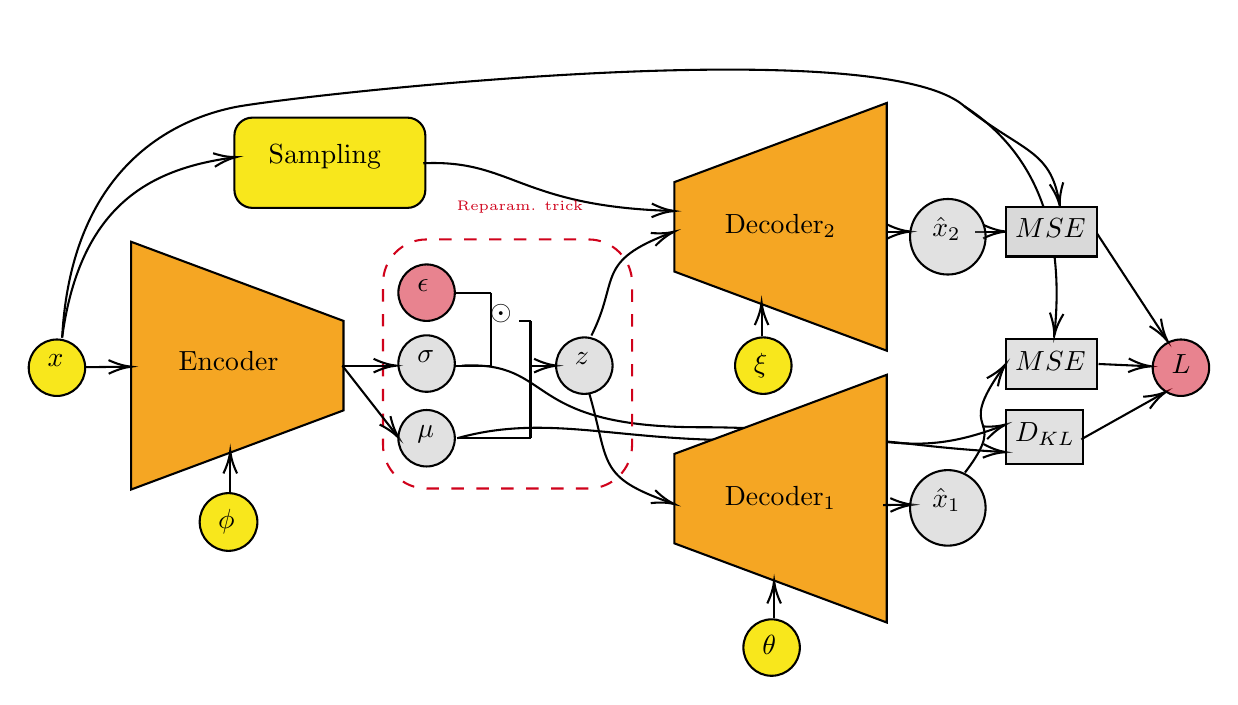
\begin{tikzpicture}[x=0.75pt,y=0.75pt,yscale=-1,xscale=1]
%uncomment if require: \path (0,300); %set diagram left start at 0, and has height of 300

%Curve Lines [id:da7098421331596159] 
\draw    (245.33,262.98) .. controls (290.33,250.33) and (325.67,265.67) .. (391.67,263.67) .. controls (457.01,261.69) and (454.72,266.57) .. (508.03,269.58) ;
\draw [shift={(509.67,269.67)}, rotate = 183.12] [color={rgb, 255:red, 0; green, 0; blue, 0 }  ][line width=0.75]    (10.93,-3.29) .. controls (6.95,-1.4) and (3.31,-0.3) .. (0,0) .. controls (3.31,0.3) and (6.95,1.4) .. (10.93,3.29)   ;
%Curve Lines [id:da69053035174273] 
\draw    (247.67,228) .. controls (293,225.67) and (275.67,257.67) .. (362.33,257.67) .. controls (448.13,257.67) and (458.47,275.96) .. (508.15,256.92) ;
\draw [shift={(509.67,256.33)}, rotate = 158.59] [color={rgb, 255:red, 0; green, 0; blue, 0 }  ][line width=0.75]    (10.93,-3.29) .. controls (6.95,-1.4) and (3.31,-0.3) .. (0,0) .. controls (3.31,0.3) and (6.95,1.4) .. (10.93,3.29)   ;
%Curve Lines [id:da21980602302822927] 
\draw    (489.67,103) .. controls (528.41,127.95) and (537.4,169.08) .. (533.2,211.72) ;
\draw [shift={(533,213.67)}, rotate = 276.15] [color={rgb, 255:red, 0; green, 0; blue, 0 }  ][line width=0.75]    (10.93,-3.29) .. controls (6.95,-1.4) and (3.31,-0.3) .. (0,0) .. controls (3.31,0.3) and (6.95,1.4) .. (10.93,3.29)   ;
%Shape: Trapezoid [id:dp5741407186499395] 
\draw  [fill={rgb, 255:red, 245; green, 166; blue, 35 }  ,fill opacity=1 ] (88.26,168.32) -- (190.56,206.44) -- (190.56,249.56) -- (88.26,287.68) -- cycle ;
%Flowchart: Alternative Process [id:dp650494001070528] 
\draw  [color={rgb, 255:red, 208; green, 2; blue, 27 }  ,draw opacity=1 ][dash pattern={on 4.5pt off 4.5pt}] (308.6,167.2) .. controls (320.2,167.2) and (329.6,176.6) .. (329.6,188.2) -- (329.6,266.2) .. controls (329.6,277.8) and (320.2,287.2) .. (308.6,287.2) -- (230.6,287.2) .. controls (219,287.2) and (209.6,277.8) .. (209.6,266.2) -- (209.6,188.2) .. controls (209.6,176.6) and (219,167.2) .. (230.6,167.2) -- cycle ;
%Shape: Trapezoid [id:dp5213418128787117] 
\draw  [fill={rgb, 255:red, 245; green, 166; blue, 35 }  ,fill opacity=1 ] (452.3,351.75) -- (350,313.63) -- (350,270.52) -- (452.3,232.4) -- cycle ;
%Straight Lines [id:da8175983884532214] 
\draw    (66,228.75) -- (86.33,228.52) ;
\draw [shift={(88.33,228.5)}, rotate = 179.36] [color={rgb, 255:red, 0; green, 0; blue, 0 }  ][line width=0.75]    (10.93,-3.29) .. controls (6.95,-1.4) and (3.31,-0.3) .. (0,0) .. controls (3.31,0.3) and (6.95,1.4) .. (10.93,3.29)   ;
%Straight Lines [id:da3169025828070092] 
\draw    (136,289.67) -- (136,271) ;
\draw [shift={(136,269)}, rotate = 90] [color={rgb, 255:red, 0; green, 0; blue, 0 }  ][line width=0.75]    (10.93,-3.29) .. controls (6.95,-1.4) and (3.31,-0.3) .. (0,0) .. controls (3.31,0.3) and (6.95,1.4) .. (10.93,3.29)   ;
%Straight Lines [id:da6211773693138245] 
\draw    (450.53,295.17) -- (463,295.02) ;
\draw [shift={(465,295)}, rotate = 179.34] [color={rgb, 255:red, 0; green, 0; blue, 0 }  ][line width=0.75]    (10.93,-3.29) .. controls (6.95,-1.4) and (3.31,-0.3) .. (0,0) .. controls (3.31,0.3) and (6.95,1.4) .. (10.93,3.29)   ;
%Straight Lines [id:da013898716368145436] 
\draw    (398.03,349.63) -- (398.03,333.63) ;
\draw [shift={(398.03,331.63)}, rotate = 90] [color={rgb, 255:red, 0; green, 0; blue, 0 }  ][line width=0.75]    (10.93,-3.29) .. controls (6.95,-1.4) and (3.31,-0.3) .. (0,0) .. controls (3.31,0.3) and (6.95,1.4) .. (10.93,3.29)   ;
%Straight Lines [id:da9591443260858074] 
\draw    (244.67,192.84) -- (261.6,192.84) ;
%Straight Lines [id:da8164735140191858] 
\draw    (244,228) -- (261.6,228) ;
%Straight Lines [id:da594124434433774] 
\draw    (261.6,192.84) -- (261.6,228) ;
%Straight Lines [id:da03926731515067883] 
\draw    (280.67,262.98) -- (245.33,262.98) ;
%Straight Lines [id:da4640907622379943] 
\draw    (280.67,206.44) -- (280.67,262.98) ;
%Straight Lines [id:da3072197400670832] 
\draw    (275.33,206.44) -- (280.67,206.44) ;
%Straight Lines [id:da3286409736096959] 
\draw    (280.67,228) -- (291.33,228) ;
\draw [shift={(293.33,228)}, rotate = 180] [color={rgb, 255:red, 0; green, 0; blue, 0 }  ][line width=0.75]    (10.93,-3.29) .. controls (6.95,-1.4) and (3.31,-0.3) .. (0,0) .. controls (3.31,0.3) and (6.95,1.4) .. (10.93,3.29)   ;
%Straight Lines [id:da5634466292060237] 
\draw    (190,228) -- (214,228) ;
\draw [shift={(216,228)}, rotate = 180] [color={rgb, 255:red, 0; green, 0; blue, 0 }  ][line width=0.75]    (10.93,-3.29) .. controls (6.95,-1.4) and (3.31,-0.3) .. (0,0) .. controls (3.31,0.3) and (6.95,1.4) .. (10.93,3.29)   ;
%Straight Lines [id:da07625676019349614] 
\draw    (190,228) -- (216.1,261.4) ;
\draw [shift={(217.33,262.98)}, rotate = 232] [color={rgb, 255:red, 0; green, 0; blue, 0 }  ][line width=0.75]    (10.93,-3.29) .. controls (6.95,-1.4) and (3.31,-0.3) .. (0,0) .. controls (3.31,0.3) and (6.95,1.4) .. (10.93,3.29)   ;
%Curve Lines [id:da3711442426235896] 
\draw    (55,214.5) .. controls (59.67,128.5) and (113.33,108.57) .. (138,103.5) .. controls (162.67,98.43) and (447,65.67) .. (489.67,103) ;
%Straight Lines [id:da25637517955917377] 
\draw    (495,163.4) -- (507.67,163.4) ;
\draw [shift={(509.67,163.4)}, rotate = 180] [color={rgb, 255:red, 0; green, 0; blue, 0 }  ][line width=0.75]    (10.93,-3.29) .. controls (6.95,-1.4) and (3.31,-0.3) .. (0,0) .. controls (3.31,0.3) and (6.95,1.4) .. (10.93,3.29)   ;
%Straight Lines [id:da31845115373615107] 
\draw    (553,163.4) -- (586.57,214.66) ;
\draw [shift={(587.67,216.33)}, rotate = 236.78] [color={rgb, 255:red, 0; green, 0; blue, 0 }  ][line width=0.75]    (10.93,-3.29) .. controls (6.95,-1.4) and (3.31,-0.3) .. (0,0) .. controls (3.31,0.3) and (6.95,1.4) .. (10.93,3.29)   ;
%Straight Lines [id:da6695013287922554] 
\draw    (554.33,227.2) -- (577.67,228.24) ;
\draw [shift={(579.67,228.33)}, rotate = 182.56] [color={rgb, 255:red, 0; green, 0; blue, 0 }  ][line width=0.75]    (10.93,-3.29) .. controls (6.95,-1.4) and (3.31,-0.3) .. (0,0) .. controls (3.31,0.3) and (6.95,1.4) .. (10.93,3.29)   ;
%Shape: Trapezoid [id:dp5535911351902126] 
\draw  [fill={rgb, 255:red, 245; green, 166; blue, 35 }  ,fill opacity=1 ] (452.3,220.8) -- (350,182.68) -- (350,139.57) -- (452.3,101.45) -- cycle ;
%Straight Lines [id:da8591062335703046] 
\draw    (452.33,163.4) -- (461.67,163.4) ;
\draw [shift={(463.67,163.4)}, rotate = 180] [color={rgb, 255:red, 0; green, 0; blue, 0 }  ][line width=0.75]    (10.93,-3.29) .. controls (6.95,-1.4) and (3.31,-0.3) .. (0,0) .. controls (3.31,0.3) and (6.95,1.4) .. (10.93,3.29)   ;
%Curve Lines [id:da6536407550801137] 
\draw    (310,213.5) .. controls (323.79,186.38) and (311.38,177.92) .. (348.28,164.04) ;
\draw [shift={(350,163.4)}, rotate = 159.91] [color={rgb, 255:red, 0; green, 0; blue, 0 }  ][line width=0.75]    (10.93,-3.29) .. controls (6.95,-1.4) and (3.31,-0.3) .. (0,0) .. controls (3.31,0.3) and (6.95,1.4) .. (10.93,3.29)   ;
%Curve Lines [id:da9597063143722228] 
\draw    (309,241.5) .. controls (318.85,275.45) and (312.53,281.49) .. (348.33,294.12) ;
\draw [shift={(350,294.7)}, rotate = 199.09] [color={rgb, 255:red, 0; green, 0; blue, 0 }  ][line width=0.75]    (10.93,-3.29) .. controls (6.95,-1.4) and (3.31,-0.3) .. (0,0) .. controls (3.31,0.3) and (6.95,1.4) .. (10.93,3.29)   ;
%Curve Lines [id:da21672448394038035] 
\draw    (489.67,103) .. controls (517.76,125.21) and (531.13,123.74) .. (535.42,149.39) ;
\draw [shift={(535.67,151)}, rotate = 261.67] [color={rgb, 255:red, 0; green, 0; blue, 0 }  ][line width=0.75]    (10.93,-3.29) .. controls (6.95,-1.4) and (3.31,-0.3) .. (0,0) .. controls (3.31,0.3) and (6.95,1.4) .. (10.93,3.29)   ;
%Curve Lines [id:da6364347511802236] 
\draw    (490,279.5) .. controls (513.1,249.14) and (482.95,264.03) .. (508.86,228.3) ;
\draw [shift={(509.67,227.2)}, rotate = 126.36] [color={rgb, 255:red, 0; green, 0; blue, 0 }  ][line width=0.75]    (10.93,-3.29) .. controls (6.95,-1.4) and (3.31,-0.3) .. (0,0) .. controls (3.31,0.3) and (6.95,1.4) .. (10.93,3.29)   ;
%Rounded Rect [id:dp2605880257934845] 
\draw  [fill={rgb, 255:red, 248; green, 231; blue, 28 }  ,fill opacity=1 ] (138,117.2) .. controls (138,112.4) and (141.9,108.5) .. (146.7,108.5) -- (221.3,108.5) .. controls (226.1,108.5) and (230,112.4) .. (230,117.2) -- (230,143.3) .. controls (230,148.1) and (226.1,152) .. (221.3,152) -- (146.7,152) .. controls (141.9,152) and (138,148.1) .. (138,143.3) -- cycle ;
%Curve Lines [id:da09251167872739519] 
\draw    (55,214.5) .. controls (63.87,148.5) and (99.9,132.96) .. (137.29,127.73) ;
\draw [shift={(139,127.5)}, rotate = 172.5] [color={rgb, 255:red, 0; green, 0; blue, 0 }  ][line width=0.75]    (10.93,-3.29) .. controls (6.95,-1.4) and (3.31,-0.3) .. (0,0) .. controls (3.31,0.3) and (6.95,1.4) .. (10.93,3.29)   ;
%Curve Lines [id:da3456156546832665] 
\draw    (229,130.5) .. controls (271.79,128.51) and (274.97,151.27) .. (348.88,153.47) ;
\draw [shift={(350,153.5)}, rotate = 181.53] [color={rgb, 255:red, 0; green, 0; blue, 0 }  ][line width=0.75]    (10.93,-3.29) .. controls (6.95,-1.4) and (3.31,-0.3) .. (0,0) .. controls (3.31,0.3) and (6.95,1.4) .. (10.93,3.29)   ;
%Straight Lines [id:da5143636758962876] 
\draw    (546,263.5) -- (585.26,241.48) ;
\draw [shift={(587,240.5)}, rotate = 150.71] [color={rgb, 255:red, 0; green, 0; blue, 0 }  ][line width=0.75]    (10.93,-3.29) .. controls (6.95,-1.4) and (3.31,-0.3) .. (0,0) .. controls (3.31,0.3) and (6.95,1.4) .. (10.93,3.29)   ;
%Straight Lines [id:da4604079869376474] 
\draw    (392,213.5) -- (392,199.5) ;
\draw [shift={(392,197.5)}, rotate = 90] [color={rgb, 255:red, 0; green, 0; blue, 0 }  ][line width=0.75]    (10.93,-3.29) .. controls (6.95,-1.4) and (3.31,-0.3) .. (0,0) .. controls (3.31,0.3) and (6.95,1.4) .. (10.93,3.29)   ;

% Text Node
\draw  [fill={rgb, 255:red, 248; green, 231; blue, 28 }  ,fill opacity=1 ]  (52.5, 229) circle [x radius= 13.6, y radius= 13.6]   ;
\draw (46.5,221.4) node [anchor=north west][inner sep=0.75pt]    {$x$};
% Text Node
\draw (109.67,219.5) node [anchor=north west][inner sep=0.75pt]   [align=left] {Encoder};
% Text Node
\draw (372.8,284.7) node [anchor=north west][inner sep=0.75pt]   [align=left] {Decoder$\displaystyle _{1}$};
% Text Node
\draw  [fill={rgb, 255:red, 155; green, 155; blue, 155 }  ,fill opacity=0.3 ]  (481.73, 165.9) circle [x radius= 18.2, y radius= 18.2]   ;
\draw (472.73,154.8) node [anchor=north west][inner sep=0.75pt]    {$\hat{x}_{2}$};
% Text Node
\draw  [fill={rgb, 255:red, 248; green, 231; blue, 28 }  ,fill opacity=1 ]  (135.17, 303.33) circle [x radius= 13.9, y radius= 13.9]   ;
\draw (128.67,295.73) node [anchor=north west][inner sep=0.75pt]    {$\phi $};
% Text Node
\draw  [fill={rgb, 255:red, 208; green, 2; blue, 27 }  ,fill opacity=0.49 ]  (230.6, 192.84) circle [x radius= 13.6, y radius= 13.6]   ;
\draw (224.6,185.24) node [anchor=north west][inner sep=0.75pt]    {$\epsilon $};
% Text Node
\draw  [fill={rgb, 255:red, 248; green, 231; blue, 28 }  ,fill opacity=1 ]  (396.83, 363.83) circle [x radius= 13.6, y radius= 13.6]   ;
\draw (390.83,356.23) node [anchor=north west][inner sep=0.75pt]    {$\theta $};
% Text Node
\draw  [fill={rgb, 255:red, 155; green, 155; blue, 155 }  ,fill opacity=0.3 ]  (230.6, 227) circle [x radius= 13.6, y radius= 13.6]   ;
\draw (224.6,219.4) node [anchor=north west][inner sep=0.75pt]    {$\sigma $};
% Text Node
\draw  [fill={rgb, 255:red, 155; green, 155; blue, 155 }  ,fill opacity=0.3 ]  (230.6, 262.98) circle [x radius= 13.6, y radius= 13.6]   ;
\draw (224.6,255.38) node [anchor=north west][inner sep=0.75pt]    {$\mu $};
% Text Node
\draw  [fill={rgb, 255:red, 155; green, 155; blue, 155 }  ,fill opacity=0.3 ]  (306.6, 228) circle [x radius= 13.6, y radius= 13.6]   ;
\draw (300.6,220.4) node [anchor=north west][inner sep=0.75pt]    {$z$};
% Text Node
\draw (259.67,196.84) node [anchor=north west][inner sep=0.75pt]    {$\odot $};
% Text Node
\draw  [fill={rgb, 255:red, 217; green, 217; blue, 217 }  ,fill opacity=1 ]  (509.67,151.4) -- (553.67,151.4) -- (553.67,175.4) -- (509.67,175.4) -- cycle  ;
\draw (512.67,155.8) node [anchor=north west][inner sep=0.75pt]    {$MSE$};
% Text Node
\draw  [fill={rgb, 255:red, 155; green, 155; blue, 155 }  ,fill opacity=0.3 ]  (509.67,249.53) -- (546.67,249.53) -- (546.67,275.53) -- (509.67,275.53) -- cycle  ;
\draw (512.67,253.93) node [anchor=north west][inner sep=0.75pt]    {$D_{KL}$};
% Text Node
\draw (243.67,147) node [anchor=north west][inner sep=0.75pt]  [color={rgb, 255:red, 208; green, 2; blue, 27 }  ,opacity=1 ] [align=left] {{\tiny Reparam. trick}};
% Text Node
\draw  [fill={rgb, 255:red, 208; green, 2; blue, 27 }  ,fill opacity=0.49 ]  (594.03, 229) circle [x radius= 13.6, y radius= 13.6]   ;
\draw (588.03,221.4) node [anchor=north west][inner sep=0.75pt]    {$L$};
% Text Node
\draw (372.8,153.4) node [anchor=north west][inner sep=0.75pt]   [align=left] {Decoder$\displaystyle _{2}$};
% Text Node
\draw  [fill={rgb, 255:red, 155; green, 155; blue, 155 }  ,fill opacity=0.3 ]  (481.73, 296.53) circle [x radius= 18.2, y radius= 18.2]   ;
\draw (472.73,285.43) node [anchor=north west][inner sep=0.75pt]    {$\hat{x}_{1}$};
% Text Node
\draw  [fill={rgb, 255:red, 155; green, 155; blue, 155 }  ,fill opacity=0.3 ]  (509.67,215.2) -- (553.67,215.2) -- (553.67,239.2) -- (509.67,239.2) -- cycle  ;
\draw (512.67,219.6) node [anchor=north west][inner sep=0.75pt]    {$MSE$};
% Text Node
\draw (153,120) node [anchor=north west][inner sep=0.75pt]   [align=left] {Sampling};
% Text Node
\draw  [fill={rgb, 255:red, 248; green, 231; blue, 28 }  ,fill opacity=1 ]  (392.83, 228) circle [x radius= 13.6, y radius= 13.6]   ;
\draw (386.83,220.4) node [anchor=north west][inner sep=0.75pt]    {$\xi $};


\end{tikzpicture}
